As the name suggests, this section has a different focus compared to the previous. This sections is concerned of classifying a few games, both in terms of gameplay and in terms of algebraic structure. This important because highlights important characteristics in underlying structure and in possible values.

This sections features a few theorems that end up proving an upper bound for the boiling point of classes of games.

\subsection*{The Result}

The temperature's upper bound results from a through analysis of the thermograph. The paper \textit{Bounding Game Temperature Using Confusion
Intervals} \cite{12} brings the first of such results, although the content featured first in Svenja Huntemann's PhD thesis \cite{5} in 2018, a year before. The proof of the boiling point requires a few smaller results and all the required content is summarized in the remaining of this subsection.

The confusion interval of a game is the range of numbers with which it is confused. A game is confused with a number if it is neither greater, smaller nor equal to that number. Any game with temperature greater than 0 is confused with numbers. Take any instance of such cases from previous sections to verify that their confusion interval includes all numbers between the points where the thermograph intersects the $t=0$ line. Some intervals also include either one or both of the intersection points, depending on what the toenail of the thermograph looks like.

However, the reader can also verify that some non-numbers with temperature 0 are also confused with numbers. Section four shows that the thermograph of \gam{0}{0} is different to that of 0, although above the $y=0$ they are the same. However, if using the surreal $\leq$ operation defined in chapter 3, one notices that $\gam{0}{0} \not\lessgtr 0$, which shows $0$ is confused with \gam{0}{0}. However, not all non-numbers behave this way, because some fall in gaps, not being confused with any number. Gaps is another delicate subject related to numbers that will not be discussed. \gam{0}{\gam{0}{0}} is a game inside a gap.

The confusion interval of \Gm{} is usually indicated by $\ell(G)$ and the intersection points are usually denoted by $LS(G)$ and $RS(G)$, and called left and right stops. Therefore $\ell(G) = LS(G)-RS(G)$. Another important definition is the thermic version of a game. The thermic version of a game \Gm{} is a game $\tilde{\Gm{}}$ with the same temperature of \Gm{} but with only one left and one right option, that are also left and right options for \Gm{}.

\textit{Theorem:} If \Gm{} is hot, then there exists a \Gm{^L} and a \Gm{^R} such that $t(G) = t(\gam{\Gm{^L}}{\Gm{^R}})$. The proof is simple: the mast of \Gm{} begins where the cooled thermographs of some of the left and right options first intersect. There are possibly many left and right options that intersect on the same point. By taking any one of them, \Gm{^{L_+}} and \Gm{^{R_+}}, it is clear that the thermic version of a game exists, because $t(G) = t(\gam{\Gm{^{L_+}}}{\Gm{^{R_+}}})$.

Finding in practice the thermic version of game is not at all simple. In fact, without additional information of \Gm{}, it would be needed to build the entire thermograph, or equivalent information, beforehand. This is an important consideration, that is also made on Dr. Huntemann thesis, but one that is not problematic. Soon, the bound will be created for \Gm{} directly, so that finding the thermic version is not necessary.

It is trivial but it is worth highlighting that the thermograph of \Gm{} and that of $\tilde{\Gm{}}$ may not be the same. In particular $\lambda_t(\tilde{\Gm{}}) \ge \lambda_t(\Gm{})$ and $\rho_t(\tilde{\Gm{}}) \leq \rho_t(\Gm{})$. If it is not clear why the observation is true: for any temperature $t$, the trajectories of the thermograph were either the maximum/minimum of all the corresponding options. The selected left and right options for the thermic version of \Gm{} are only the minimum/maximum for temperatures close to the boiling. Therefore the initial trajectory might be different, but is always lesser/greater or equal to the thermic trajectories.

Using the notation described above it may be simpler. $\lambda_t(\Gm{}) = LS(\Gm{_t}) = max_{\Gm{^L}}(RS(\Gm{^L_t}) - t)$. Since $\Gm{^{L_+}} \in \Gm{^L}$, it is clear that $\lambda_t(\tilde{\Gm{}}) \ge \lambda_t(\Gm{})$. An equivalent statement can be made for the right trajectory.

A result, when fixating $t=0$ is:

\begin{align*}
\ell(\tilde{\Gm{}}) \leq& \ell(\Gm{})\\
\text{Since } \ell(\tilde{\Gm{}}) = LS(\tilde{\Gm{}}) - RS(\tilde{\Gm{}})\leq& LS(\Gm{}) - RS(\Gm{}) = \ell(\Gm{})
\end{align*}

The thermograph, as described in the previous section, is composed of straight lines and $\pm$45$\deg$ oblique lines. The bound is based on this and the size of the confusion interval. Before proceeding, one additional definition.

Let $T^L$ be the sequence $(0, t_1, t_2, \ldots, t_k)$ of the temperatures of the turning points of $\lambda(\tilde{\Gm{}})$. Let, now, $A^L$ be the sequence $(a_0, a_1, \ldots, a_k)$ of labels given by:

\hspace{2cm}$
\begin{cases}
a_i $ is \textit{vertical} if $ \rho(\tilde{\Gm{}}^L_{t_{i+1}}) = \rho(\tilde{\Gm{}}^L_{t_i})\\
a_i $ is \textit{oblique} if $ \rho(\tilde{\Gm{}}^L_{t_{i+1}}) < \rho(\tilde{\Gm{}}^L_{t_i})
\end{cases}
$

Lastly,

\hspace{2cm} $T^L_{\text{V}} = \sum\limits_{\substack{i\;|\;a_i \text{ is} \\ \text{vertical}}}(t_{i+1} - t_i)$

\hspace{2cm} $T^L_{\text{O}} = \sum\limits_{\substack{i\;|\;a_i \text{ is} \\ \text{oblique}}}(t_{i+1} - t_i)$

Notice that the right counterpart can be done similarly. Essentially, $T^L_{\text{V}}$ is the length of the vertical segments and $T^L_{\text{O}}$ is the length of the oblique segments. Of course

\begin{align*}
	t(\Gm{}) =& T^L_{\text{V}} + T^L_{\text{O}}.\\
	&\text{and} \\
	\ell(\tilde{\Gm{}}) =& T^L_{\text{O}} + T^R_{\text{O}}.
\end{align*}

\textit{The theorem} is the following:

Given \Gm{} and $\tilde{\Gm{}}$ its thermic version, then

$$
t(\Gm{}) \leq \ell(\Hm) + \frac{\ell(\Gm{})}{2}
$$

where $\Hm = \tilde{\Gm{}}^L$ if $T^L_V \ge T^R_V$, otherwise $\Hm = \tilde{\Gm{}}^R$. For simplicity, the proof considers that $\Hm = \tilde{\Gm{}}^L$, but again, an equivalent procedure proves the other case.

The length of $T^L_V$ is at most the length of the oblique segments of $\rho(\tilde{\Gm{}}^L)$. Notice that it could be smaller because the left and right options might intersect before the mast of $\tilde{\Gm{}}^L$. In any case, it is clear that the length of this oblique segments is at most the same size of the confusion interval of$\tilde{\Gm{}}^L$. It could be smaller in case there are oblique segments in $\lambda(\tilde{\Gm{}}^L)$.

Therefore, $T^L_V \leq \ell(\tilde{\Gm{}}^L)$

Additionally:

\begin{align*}
T^L_V + T^L_O =&\;T^R_V+T^R_O\\
\text{Since, in this case, }& T^L_V \ge T^R_V\text{:}\\
T^L_O \leq&T^R_O
\end{align*}

Therefore:

\begin{align*}
	2\times T^L_O \leq T^L_O + T^R_O =&\;\ell(\tilde{\Gm{}}) \leq \ell(\Gm{})\\
	T^L_O = \frac{\ell(\tilde{\Gm{}})}{2} &\leq \frac{\ell(\Gm{})}{2}
\end{align*}

Resulting in:

$$
t(G) = T^L_V + T^L_O \leq \ell(\tilde{\Gm{}}^L) + \frac{\ell(G)}{2}
$$

Although longer than other proofs in this text, it is yet another simple proof. The equations and the many symbols might make it unclear, but the each o f the steps can be visualized. For clarification, it follows an explanation of the starting points of each sequence or equations \todo{improve clarification?}.

$T^L_V + T^L_O =\;T^R_V+T^R_O$ is straight forward, because what defines the height is the intersection point of left and right, which is the same for both trajectories. $2\times T^L_O \leq T^L_O + T^R_O$ is a direct result of the previous inequation. 

This theorem uses the thermic version of games, which, again, are hard to find in itself. However, from this version, another result that does not use the thermic versions is possible.

\textit{The theorem} might be re-written as:

Let n, m two non-negative numbers. If $S$ is class of games such that for all $G \in S,\;\ell(G) \leq n$ and for all options $\ell(G^{L/R}) \leq m$, then:

$$
BP(S) \leq \frac{n}{2} + m
$$

Although immediate, deciding whether the first version implies the version above might require an explanation. $t(G) \leq \ell(\tilde{\Gm{}}^L) + \frac{\ell(G)}{2} \leq \frac{n}{2} + \ell(\tilde{\Gm{}}^L)$ is true because $\forall G \in S,\;\ell(G) \leq n$. Since $\ell(G^{L/R}) \leq m$, then $\ell(\tilde{\Gm{}}^L) \leq m$, which implies the last inequation $t(G) \leq \frac{n}{2} + \ell(\tilde{\Gm{}}^L) \leq \frac{n}{2} + m$.

Using a class of games is not as straight forward as using the definitions typically used in this text. To idea to use the theorem is to first create a class, following the restrictions - therefore having a bound for the temperature. Then one should prove a game or a pattern of games belong to this class, to make use of this bound.

Let, for example, the class $S$ to be defined by $\{G : \ell(G)\leq100, \ell(G^L)\leq200, \ell(G^R)\leq200\}$. Since $S$ meets the requirements it has the proposed boiling point. $\forall G \in S, BP(G) \leq 250$. The maximum length of the confusion intervals are so large that, in particular, all games of this text belong to $S$. It is possible to verify that all the temperatures of games instanced in the text are indeed smaller than $250$ \todo{maybe remove this comment}. In fact the hottest game \Gm{} analyzed in this text was:

\begin{center}
	\begin{tikzpicture}
		\begin{scope} []
			\draw[fill=yellow] (-1,-1) rectangle ++(8,1.9);
			\node[circle, draw, fill=purple2] at (0,0) {7 $|$ {-}9};
			\node[circle, draw, fill=purple2] at (2,0) {28 $|$ {-}4};
			\draw[thick] (3,-0.75) -- (3,0.75);
			\node[circle, draw, fill=purple2] at (4,0) {{-}3 $|$ 1};
			\node[circle, draw, fill=purple2] at (6,0) {2 $|$ 22};
		\end{scope}
	\end{tikzpicture}
\end{center}

With, as shown before, the thermograph:
\begin{center}
	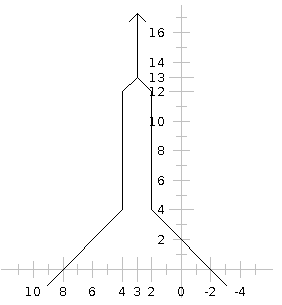
\includegraphics[scale=0.5]{../images/thermA.png}
\end{center}

In this case, $\ell(G) = 10 \leq 100$ and $\ell(\Gm{^{L_1}}) = \ell(\Gm{^{R_1}}) = 0 \leq 200$ and $\ell(\Gm{^{L_2}}) = \ell(\Gm{^{R_2}}) = 24 \leq 200$. The boiling point bound the theorem provided for $S$ is loose for \Gm{}. However, it is unclear if that is because the confusion intervals that define the class are also too lose or if the bound itself is large.

Let $S_*$, now, be the class given by $\{G : \ell(G)\leq10, \ell(G^L)\leq24, \ell(G^R)\leq24\}$. From the analysis of the previous paragraph, \Gm{\in S_*}. However, in this case, the confusion intervals of \Gm{} are tight in respect to the ones that define the class. From the theorem $\forall G \in S_*,\; BP(G) \leq 29$. The bound is tighter for \Gm{} but is still loose, which may lead to the belief that this bound is loose in general.

In order to verify whether the bound is in fact loose, it would bee needed to show the following, or something similar:
$$
\forall S,\;\exists x\in SN,\; x>0\;|\; \underset{G\in S}{max}BP(G) \leq BP(S) + x
$$

To dismiss the idea, however, it could be shown:
$$
\exists G \in S_*\;|\;\not\exists x>0,\; BP(G)\leq BP(S)+x
$$

Starting out with the previous example, take $\tilde{G} = \gam{\gam{28}{4}}{\gam{2}{-22}}$. The temperature is, of course, the same as before, 13. However, the Left and Right slant may be moved, since $\ell(\tilde{G}) = 2$. Take \Gm{_+=\gam{\gam{36}{12}}{\gam{2}{-22}}}, result of shifting the left slant to the left, while maintaining the left confusion interval.

\begin{center}
\begin{tabular}{cc}
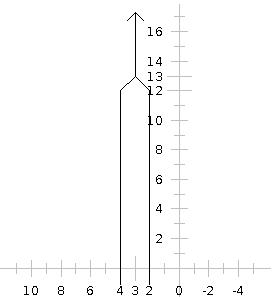
\includegraphics[scale=0.5]{../images/gtherm.png} & 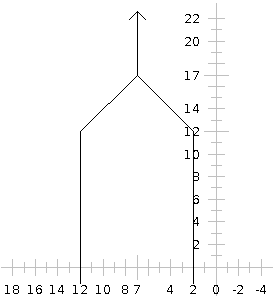
\includegraphics[scale=0.5]{../images/gplus.png} \\
$\tilde{G}$ & \Gm{_+} \\
\end{tabular}
\end{center}

The temperature 17 is higher than the initial one but is still far away from the desired 29. However, it is still possible to increase it more. The boiling point of left and right slants are 12, and, for this reason, the oblique line in the thermograph start at $t=12$. Making the left and right games hotter would increase the overall temperature, but increasing the confusion interval is not allowed as it is desired that the resulting game belongs to the class $S_*$.

Since the thermographs of \Gm{^{L/R}} are made of two oblique lines, making part of the lines straight would increase their temperature. One way of doing it is changing \Gm{^L} to \gam{\gam{60}{36}}{12}. The temperature of
\Gm{_-=\gam{\gam{\gam{60}{36}}{12}}{\gam{2}{\gam{-22}{-46}}}} is 23. To simplify further analysis, take \Gm{_1 = \gam{\gam{\gam{53}{29}}{5}}{\gam{{-}5}{\gam{-29}{-53}}}}, result of centering \Gm{_-} at 0. Notice that \Gm{_1 = \pm\gam{\gam{53}{29}}{5}}.

\begin{center}
	\begin{tabular}{cc}
		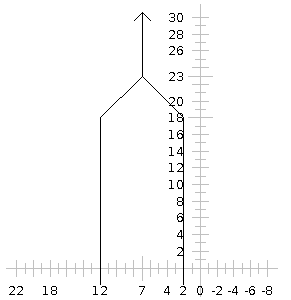
\includegraphics[scale=0.5]{../images/gminus.png} & 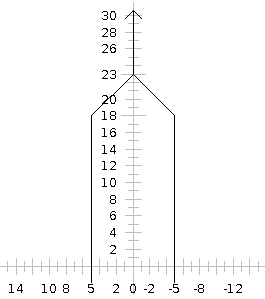
\includegraphics[scale=0.5]{../images/gone.png} \\
		\Gm{_-} & \Gm{_1} \\
	\end{tabular}
\end{center}

Following the idea of making one of the slants of \Gm{^{L/R}} straighter in order to increase their temperature, it is possible to keep increasing the temperature of \Gm{}. Consider the following sequence of games is $S_*$:

\begin{center}
	\begin{tabular}{c|c|c}
		i & \Gm{} & $t(G)$	\\
		\hline
		0 & $\pm$ \gam{29}{5} & 17 \\
		1 & $\pm$ \gam{\gam{53}{29}}{5} & 23 \\
		2 & $\pm$ \gam{\gam{\gam{77}{53}}{29}}{5} & 26 \\
		3 & $\pm$ \gam{\gam{\gam{\gam{101}{77}}{53}}{29}}{5} & 27.5 \\
	\end{tabular}\\
	\vspace{0.3cm}$\cdots$
\end{center}

The result that the temperature of games in this sequence increases and converges to 29 is desired, but it must be proved. The following proof is general for all sequence of games made in the likes of the sequence above.

\textit{Proof:} \todo{I made the proof -- revise}
\begin{list}{}{}
	\item[$\rightarrow$] Each term of the sequence increases the length of the straight segment of the left option of \Gm{^L} by $\frac{\ell(G^L)}{2^{i+1}}$.
	\item[ ] [Via Induction]
	\item[ ] Base case: $i=1$. Let $\Gm{=\gam{\gam{a + 2\ell(G^L)}{a+\ell(G^L)}}{a}}$. The right trajectory, $\rho$, of \gam{a + 2\ell(G^L)}{a+\ell(G^L)} is oblique until $t=\frac{\ell(G^L)}{2}$. Therefore the left trajectory, $\lambda$, of \Gm{} is straight until $\frac{\ell(G^L)}{2}$. At $t=\frac{\ell(G^L)}{2}$, the right trajectory is at the $a + \frac{\ell(G^L)}{2}$ x-coordinate. Since both trajectories are oblique above this temperature, they cross at the point $(a + \frac{3\ell(G^L)}{4},\; \frac{3\ell(G^L)}{4})$. Therefore, temperature was increased by $\frac{\ell(G^L)}{2}$.
	\item[ ] Induction Hypothesis: $i=k$. Let 
	$$
	\Gm{=\gam{
			\gam{
				\gam{
					\gam{\ldots
						\gam
							{a + (k+1)\ell(G^L)}
							{a + k\ell(G^L)}
						}
						{\ldots}
					}
					{a + 2\ell(G^L)}
				}
				{a+\ell(G^L)}
			}
			{a}
		}
	$$
	Let $b = a + \ell(G^L)$. It is possible to rewrite $G$ so that:
	$$
	\Gm{=\gam{
			\gam{
				\gam{
					\gam{\ldots
						\gam
						{b + k\ell(G^L)}
						{b + (k-1)\ell(G^L)}
					}
					{\ldots}
				}
				{b+\ell(G^L)}
			}
			{b}
		}
		{a}
	}
	$$
	Using the inductive hypothesis on:
	$$
	\Hm{=
			\gam{
				\gam{
					\gam{\ldots
						\gam
						{b + k\ell(G^L)}
						{b + (k-1)\ell(G^L)}
					}
					{\ldots}
				}
				{b + \ell(G^L)}
			}
			{b}
	}
	$$
	The left slant of $\Hm^L$ has a straight segment of size $\sum\limits_{i=1}^{k-1} \frac{\ell(G^L)}{2^{i+1}}$. Since the right option of $H^L$ is a number, $BP(H^L)= \sum\limits_{i=1}^{k-1} \frac{\ell(G^L)}{2^{i+1}} + \frac{\ell(G^L) - \sum\limits_{i=1}^{k-1} \frac{\ell(G^L)}{2^{i+1}}}{2}$. Therefore, $BP(H^L)= \frac{\ell(G^L) + \sum\limits_{i=1}^{k-1} \frac{\ell(G^L)}{2^{i+1}}}{2} = \sum\limits_{i=1}^{k} \frac{\ell(G^L)}{2^{i+1}}$. Since the right slant of $H^L$ is oblique with size equals to the given temperature, then the left slant of $H$ is straight with the same size. Since $H = G^L$, then the inductive step is indeed correct.
	\item[$\rightarrow$] Each term of the sequence increases the length of the straight segment of the right option of \Gm{^R} by $\frac{\ell(G^R)}{2^{i+1}}$.
	\item[ ] The proof is analogous.
	\item[$\rightarrow$] If both the left option of \Gm{^L} and the right option of \Gm{^R} have their straight length increased by $l$, then so does \Gm{}.
	\item[ ] As seen before, $t(G) = T^L_V + T^L_O$. Since $\forall i,\; G_i = \tilde{G_i}$ and that increasing both trajectories straight segments does not affect the size of the oblique segments, it is possible to conclude that the temperature of the whole game will increase exactly $l$. Since, again, the size of the oblique segment does not change than the size of the straight segment increased by $l$.
	\item[$\rightarrow$] The temperature of the games in this sequence converges to the proposed boiling point, while always being elements of the initial class $S$.
	\item[ ] Notice that $RS(G^L)$ and $LS(G^R)$ remain the same across all iterations, and that $RS(G^L) - LS(G^R) = \ell(G)$, it is clear that $\forall i, \ell(G_i) = \ell(G)$.
	\item[ ] Notice that the observation above is valid for \Gm{^L} and \Gm{^R}.
	\item[ ] The previous two observations show that every game in the sequence belongs to $S$.
	\item[ ] The initial height is $\frac{\ell(G)}{2} + \frac{\ell(G^L)}{2}$. From the first three points of the proof, at each iteration $i$ the straight segments of $\lambda(G)$ and $\rho(G)$ increase by $\frac{\ell(G^L)}{2^{i+1}}$, $\ell(G^L) = \ell(G^R)$. Since increasing the straight segments of $\lambda(G)$ and $\rho(G)$ does not affect the size of the oblique segments, then $t(G)$ increases by that amount at each iteration.
	\item[] \hspace{-1cm} $t(G_k) = \frac{\ell(G)}{2} + \frac{\ell(G^L)}{2} + \sum\limits_{i=1}^{k} \frac{\ell(G^L)}{2^{i+1}} = \frac{\ell(G)}{2} + \sum\limits_{i=1}^{k} \frac{\ell(G^L)}{2^{i}} = \frac{\ell(G)}{2} + \ell(G^L) - \frac{\ell(G^L)}{2^k} \leq \frac{\ell(G)}{2} + \ell(G^L)$.
\end{list}

The sequence of games, then, shows that the given bound is not loose. In fact, it shows that the bound is optimal for some cases. It is worth mentioning that, although this section follows the aforementioned paper, the proof above is original. The paper does convey the strategy and the regard about the optimality of the bound but the proof of convergence is skipped. Although long and with many symbols, the proof is quite simple and might be considered trivial.

An interesting way to complete and put to practice the analysis of the theorem is to show it can be used to characterize a pattern of domineering boards. To use the bound all games following the pattern must belong to a class, based on the confusion interval restrictions, like before.

When bounding `$2\times n$ snakes' boards, the thesis and the featured papers diverge. Probably in the year between the publish of the thesis and the paper the technique was refined, resulting in the thesis bringing a bound of $5$ to the temperature and the paper reducing it to $3$. The proof brought to this text will show the point of divergence. Before showing the proof, another necessary definition and lemma are provided.

A `snake' board, same adjective used in ``Kim's snakes" from the previous chapter, is a board without any $2\times 2$ subgrid. A `$2\times n$' snake is a snake that fits in a $2\times n$ board. It is possible to use the term `snake fitting in a $2\times n$ board', and this means that the board is a snake that can be folded such that it becomes a `$2\times n$' snake with the same value.

The lemma is: Let $\epsilon$ be any infinitesimal and \Gm{} be a hot game. If for all left options \Gm{^L}, $n$ is a number such that $G^L - G - n +\epsilon \leq 0$, then $\ell(G) \leq n$. The proof is simple, again.
\begin{align*}
	\ell(G) =& LS(G) - RS(G) \\
	=& RS(G^L) + LS(-G) \\
	\leq& LS(G^L - G) \\
	\leq& n
\end{align*}

It is clear that $LS(G) = RS(G^L),\; RS(G) = - LS(-G)$, but the second equation is there to help visualize the first inequation. The last inequation is true because $G^L - G + \epsilon \leq n \longrightarrow LS(G^L-G)\leq n$, explained amid the discussion in the beginning of this section. The first inequation is true because $G^L - G = \gam{G^{LL}-G^L}{G^{LR}-G^R}$, meaning that $LS(G^L-G)$ derives from a game $\Hm = \Gm{^L_+} - \Gm{_-}$. In particular, it is possible to take \Gm{^L_+} to be a game that defines the right stop for \Gm{^L} and $-\Gm{_-}$ the game that defines the left stop for $-G$, and, therefore, the inequality is true.

The meaning of this lemma is that if it is possible to bound the value of the game to the left, or to positive side, then it is possible to bound the confusion interval. This is a weaker result compared to the previous but it is one that connects the stops with the confusion interval so it is extremely useful.

Now it is possible to characterize some domineering boards. \textit{The temperature of snakes fitting a $2\times n$ board is at most $3$.} The proof consists of showing that $\ell(G), \ell(G^L), \ell(G^R) \leq 2$, by the means of showing that for $\Hm = G \lor G^L \lor G^R \rightarrow H^L -H -2 \leq 0$ and using the lemma above.

Considering the case $H = G^R$, \Hm is a two component board, so it is possible to separate them in distinct games. Let $-H = -G^R = -G_1 - G_2$. $H^L$ on the other hand is \Gm{^R} with the addition of a left move. The only cases a left move does not exist in \Gm{^R} is if \Gm{} is one of the following:

\begin{figure} [!ht]
\begin{center}
\begin{tikzpicture}
\draw[] (0,0) rectangle ++(0.3,0.3);
\draw[] (0,0.3) rectangle ++(0.3,0.3);
\end{tikzpicture}
\hspace{1cm}
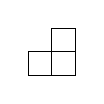
\begin{tikzpicture}
	\draw[] (0,0) rectangle ++(0.3,0.3);
	\draw[] (-0.3,0) rectangle ++(0.3,0.3);
	\draw[] (0,0.3) rectangle ++(0.3,0.3);
\end{tikzpicture}
\hspace{1cm}
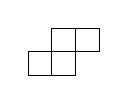
\begin{tikzpicture}
	\draw[] (0,0) rectangle ++(0.3,0.3);
	\draw[] (-0.3,0) rectangle ++(0.3,0.3);
	\draw[] (0,0.3) rectangle ++(0.3,0.3);
	\draw[] (0.3,0.3) rectangle ++(0.3,0.3);
\end{tikzpicture}
\end{center}
\end{figure}

In all the cases above, the temperature is below 3, so it is not a problem. Without losing generality, let \Gm{_1} be a component where there is a right move, and let the initial left move be any such move in \Gm{_1}, therefore, $H^L = G_1^L + G_2$. Now it is clear that this case can be reduced to the case $H = G_*$, with \Gm{_*} a smaller board than \Gm{}:

$$
H^L - H = G_1^L + G_2 - G_1 - G_2 = G_1^L - G_1
$$

Repeating the process with $H = G^L$, $-H = -G^L = -G_1 - G_2$ and $H^L = G_1^L + G_2$. The only cases \Gm{_1^L} does not exist is if
\Gm{=\begin{tikzpicture}
		\draw[] (0,0) rectangle ++(0.3,0.3);
		\draw[] (0.3,0) rectangle ++(0.3,0.3);
	\end{tikzpicture} \text{ or } 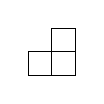
\begin{tikzpicture}
	\draw[] (0,0) rectangle ++(0.3,0.3);
	\draw[] (0.3,0) rectangle ++(0.3,0.3);
	\draw[] (0.3,0.3) rectangle ++(0.3,0.3);
\end{tikzpicture}} and both of them have temperature lesser than 3. Again it is clear that this case can also be reduced to the case $H = G_*$:

$$
H^L - H = G_1^L + G_2 - G_1 - G_2 = G_1^L - G_1
$$

Therefore, if $\ell(G) \leq 3$ then the confusion interval of both option are also smaller than 3. To prove that $G^L - G - 2 \leq 0$ it is shown a winning strategy for right in $G^L - G - 2$, which shows that the position is negative. First notice that $-G$ is \Gm{} flipped so that it fits in a $n\times 2$ board, but a useful way, that is used in this proof, to consider $-G$ is Left playing on the horizontal and Right playing on the vertical.

To help visualize the strategy for this case, let the `shadow' of a move be the same cells that the move occupied, but in the opposing board. Also the board resultant from play in $G^L$ is called the original board and the board resultant from play in $-G$ is called the opposing board. For instance:

\begin{figure}[h]
	\centering
	\begin{subfigure}{0.17\linewidth} \centering
		\begin{tikzpicture}
			\node (title) at (0.45,1) {\Gm{^{L/R}}};
			\draw[] (0,0) rectangle ++(0.3,0.3);
			\draw[fill=gray] (0.3,0.3) rectangle ++(0.3,0.3);
			\draw[] (0.6,0.3) rectangle ++(0.3,0.3);
			\draw[fill=gray] (0.3,0) rectangle ++(0.3,0.3);
			\node[] at (1.3,0.3){$\cdots$};
			\node[] at (-0.4,0.3){$\cdots$};
		\end{tikzpicture}
		\caption*{\hspace{0.1cm}Orginal move\newline Original board}
	\end{subfigure}
	\hspace{1cm}
	\begin{subfigure}{0.17\linewidth} \centering
		\begin{tikzpicture}
			\node (title) at (0.45,1) {-$G$};
			\draw[] (0,0) rectangle ++(0.3,0.3);
			\draw[pattern=north west lines,pattern color=gray] (0.3,0.3) rectangle ++(0.3,0.3);
			\draw[] (0.6,0.3) rectangle ++(0.3,0.3);
			\draw[pattern=north west lines,pattern color=gray] (0.3,0) rectangle ++(0.3,0.3);
			\node[] at (1.3,0.3){$\cdots$};
			\node[] at (-0.4,0.3){$\cdots$};
		\end{tikzpicture}
		\caption*{\hspace{0.15cm}Shadow move\newline Opposing board}
	\end{subfigure}
\end{figure}

In the game $G^L -G -2$, if Right plays first, he/she simply has to mimic each and every move Left made by playing the shadow move, maintaining $-2$ intact, starting with the move already played in \Gm{^L}. If, instead Left goes first, he/she can play one of two options. The first is to play a move that does not intersect the shadow of the previous move. In this case, right must play the shadow of either the first or the second move.

Essentially, this first case maintains the original conditions while reducing the board size. This case leads $G^{L_*} -G -2$ to $G^{L_*L} -G^{L_*} -2$, which, by taking $H = G^{L_*}$, is $H^{L} -H -2$. Therefore the only worrisome Left move is one that intersects the shadow of the initial move. This move is not exactly the shadow move because in the opposing board Left moves in another orientation. After Left's move, Right must move on the $-2$ component, taking it to $-1$.

Now, Left can, again, play a move that does not intersect any of the shadows, but this would be met by the same strategy as before, so Left must play a move that intersects a shadow. However, Left cannot move intersecting the shadow of the previous move, because the initial move would be adjacent to this third move and since the mover are both vertical, a $2\times 2$ subgrid would have to exist. The only shadow Left can intersect is that of the first move, playing on the opposing component again. After Left's third move, right plays on the $-1$ component.

At this time, Left can no longer play on any shadows, so he/she cannot avoid Right's strategy and will eventually lose. Therefore, if \Gm{} is a snake fitting in a $2\times n$ grid, then $G^L - G -2 < 0$. This means that $\ell(G),\ell(G^L),\ell(G^R) \leq 2$. By using the bound result, in turn, it means that $t(G) \leq 3$. 

This result from the 2019 paper is different, as stated before, from the 2018 thesis because the first part of the proof, that shows the cases $H=G^L,G^R$ can be reduced to the case $H=G$, was missing. Instead the original text only showed that the confusion intervals of $G^L,G^R$ were smaller than 4. This second result is clear because both $G^L$ and $G^R$ are made of two components that are snakes fitting in $2\times n$ grids. As the text shows that such a snake has the confusion interval smaller or equal to 2, then two snakes have that interval smaller or equal to 4.














